\documentclass[a4paper,14pt]{extarticle}

\usepackage[utf8x]{inputenc}
\usepackage[T1,T2A]{fontenc}
\usepackage[russian]{babel}
\usepackage{hyperref}
\usepackage{indentfirst}
\usepackage{here}
\usepackage{array}
\usepackage{graphicx}
\usepackage{caption}
\usepackage{subcaption}
\usepackage{chngcntr}
\usepackage{amsmath}
\usepackage{amssymb}
\usepackage{pgfplots}
\usepackage{pgfplotstable}
\usepackage[left=2cm,right=2cm,top=2cm,bottom=2cm,bindingoffset=0cm]{geometry}
\usepackage{multicol}

\renewcommand{\le}{\ensuremath{\leqslant}}
\renewcommand{\leq}{\ensuremath{\leqslant}}
\renewcommand{\ge}{\ensuremath{\geqslant}}
\renewcommand{\geq}{\ensuremath{\geqslant}}
\renewcommand{\epsilon}{\ensuremath{\varepsilon}}
\renewcommand{\phi}{\ensuremath{\varphi}}

\counterwithin{figure}{section}
\counterwithin{equation}{section}
\counterwithin{table}{section}
\newcommand{\sign}[1][5cm]{\makebox[#1]{\hrulefill}} % Поля подписи и даты
\graphicspath{{pics/}} % Путь до папки с картинками
\captionsetup{justification=centering,margin=1cm}
\def\arraystretch{1.3}

\begin{document}

\begin{titlepage}
\begin{center}
	\textbf{Санкт-Петербургский Политехнический Университет \\Петра Великого}\\[0.3cm]
	\small Институт компьютерных наук и технологий \\[0.3cm]
	\small Кафедра компьютерных систем и программных технологий\\[4cm]
	
	\textbf{ОТЧЕТ}\\ \textbf{о лабораторной работе}\\[0.5cm]
	\textbf{<<Исследование частотных характеристик пассивных RC-цепей>>}\\[0.1cm]
	\textbf{Электротехника и Электроника}\\[10.5cm]
\end{center}

\begin{flushright}
	\begin{minipage}{0.60\textwidth}
		\begin{flushleft}
			\small \textbf{Работу выполнили студенты}\\[3mm]
			\small группа 23501/4 \hspace*{17mm} Дьячков В.В.\\[3mm]
			\small группа 23501/4 \hspace*{17mm} Ламтев А.Ю.\\[5mm]
			
			\small \textbf{Преподаватель}\\[5mm]
		 	\small \sign[3.5cm] \hspace*{8mm} к.т.н., доц. Кочетков Ю.Д.\\[0.5cm]
		\end{flushleft}
	\end{minipage}
\end{flushright}

\vfill

\begin{center}
	\small Санкт-Петербург\\
	\small \the\year
\end{center}
\end{titlepage}

\section{Цель работы}

Приобретение навыков настройки и исследования импульсных генераторов (автоколебательных и ждущих), определения областей применения различных интегральных микросхем в генераторах.

\section{Чертеж схемы исследуемого устройства}

\begin{figure}[H]
\begin{center}
	\begin{subfigure}[b]{0.35\textwidth}
		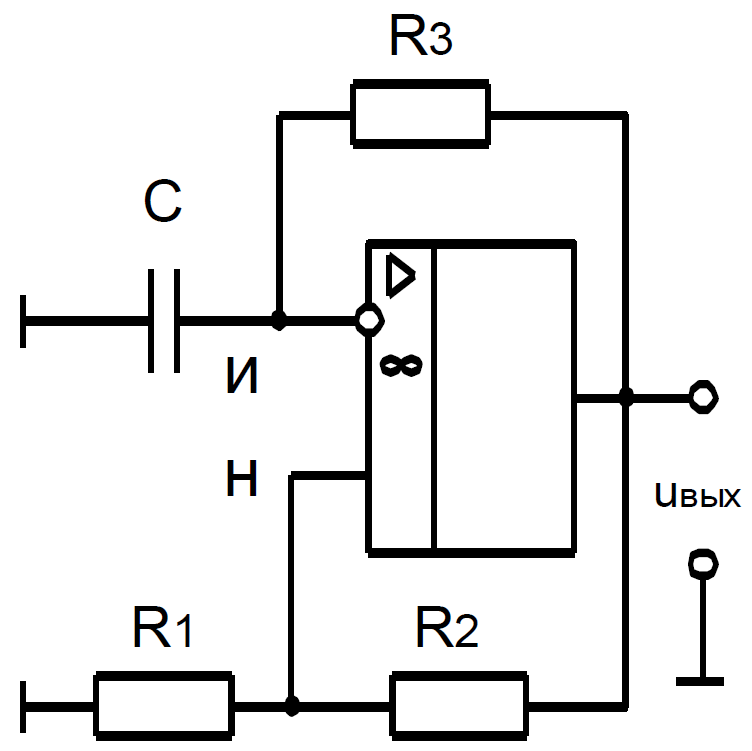
\includegraphics[scale=0.3]{scheme1}
		\caption{Симметричный мультивибратор}
	\end{subfigure}
	~
	\begin{subfigure}[b]{0.35\textwidth}
		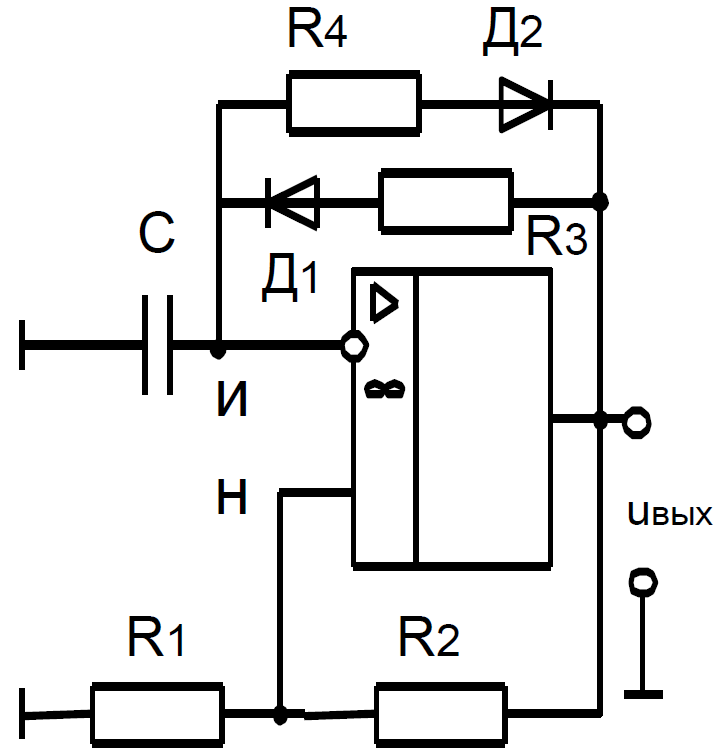
\includegraphics[scale=0.3]{scheme2}
		\caption{Несимметричный мультивибратор}
	\end{subfigure}
	~
	\begin{subfigure}[b]{0.35\textwidth}
		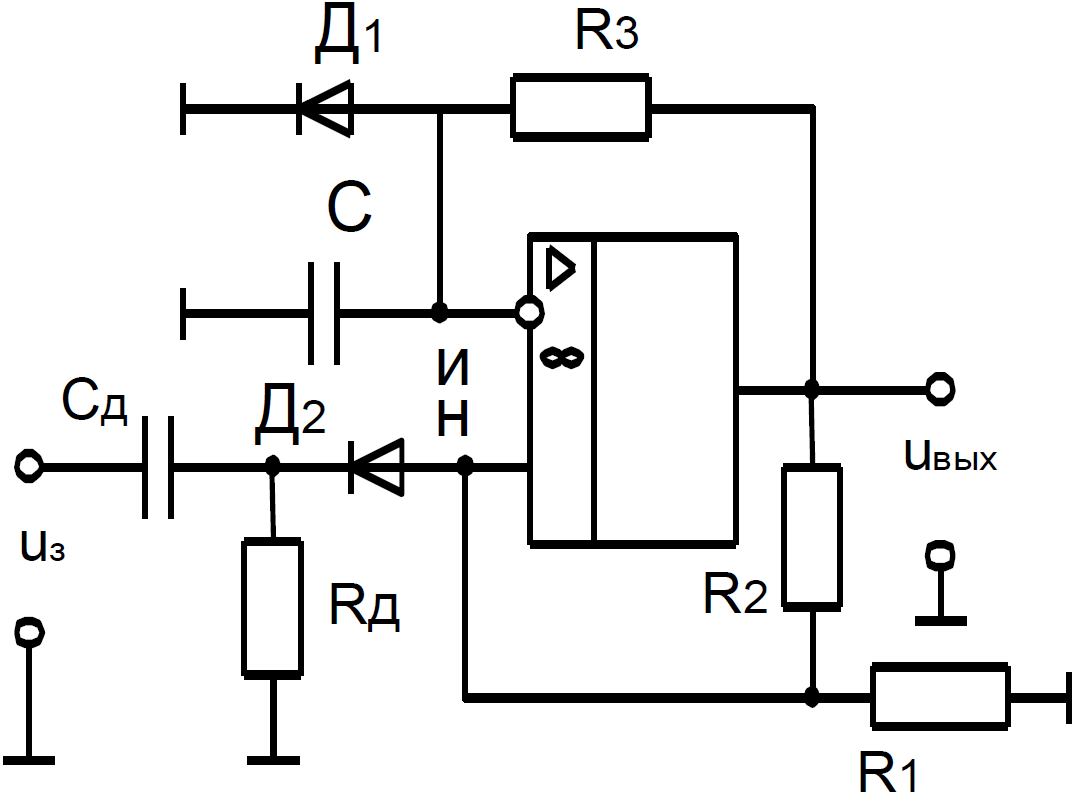
\includegraphics[scale=0.3]{scheme3}
		\caption{Ждущий генератор}
	\end{subfigure}
	\caption{}
\end{center}
\end{figure}


\section{Исходные данные}

Операционный усилитель \verb+К140УД6+.

\begin{table}[H]
\begin{center}
	\caption{Исходные данные}
	\def\tabcolsep{10pt}
	\begin{tabular}{|c|c|c|c|c|c|c|c|}
		\hline
		$t_{\text{и1}}$, мкс &
		$t_{\text{и2}}$, мкс &
		$K_{\text{Д}}$ &
		$C$, нФ &
		$R_{\text{Д}}$, кОм &
		$C_{\text{Д}}$, пФ &
		$E_{01}$, В &
		$E_{02}$, В \\
		\hline
		20 &
		40 &
		1 &
		3 &
		10 &
		1500 &
		15 &
		-15 \\
	    \hline	
	\end{tabular}
\end{center}
\end{table}

\section{Теоретические расчёты}

\subsection{Расчет параметров элементов}

\section{Экспериментально снятые зависимости}

\section{Погрешности}

\section{Выводы}

Приведённые погрешности полученных в ходе эксперимента значений $K_1$, $K_2$ и $K_3$ не превышают превышают предельно допустимые погрешности.

Таким образом, формулы \ref{eq:4:1} -- \ref{eq:4:5} являются верными.

\end{document}